%%
%% Beginning of file 'sample.tex'
%%
%% Modified 2015 December
%%
%% This is a sample manuscript marked up using the
%% AASTeX v6.x LaTeX 2e macros.

%% AASTeX is now based on Alexey Vikhlinin's emulateapj.cls 
%% (Copyright 2000-2015).  See the classfile for details.
%%
%% AASTeX requires revtex4-1.cls (http://publish.aps.org/revtex4/) and
%% other external packages (latexsym, graphicx, amssymb, longtable, and epsf).
%% All of these external packages should already be present in the modern TeX 
%% distributions.  If not they can also be obtained at www.ctan.org.

%% The first piece of markup in an AASTeX v6.x document is the \documentclass
%% command. LaTeX will ignore any data that comes before this command. The 
%% documentclass can take an optional argument to modify the output style.
%% The command below calls the preprint style  which will produce a tightly 
%% typeset, one-column, single-spaced document.  It is the default and thus
%% does not need to be explicitly stated.
%%

%% using aastex version 6
\documentclass[onecolumn]{aastex6}
\usepackage{subfigure}
\usepackage{amsmath}

%% The other main article choice is a tightly typeset, two-column article
%% that more closely resembles the final typeset pdf article.
%%
%% \documentclass[twocolumn]{aastex6}
%% 
%% There are other optional arguments one can envoke to allow other 
%% actions. 
%%
% These are the available options:
%   manuscript	: onecolumn, doublespace, 12pt fonts
%   preprint	: onecolumn, single space, 10pt fonts
%   preprint2	: twocolumn, single space, 10pt fonts
%   twocolumn	: a two column article. Probably not needed, but here just in case.
%   onecolumn	: a one column article; default option.
%   twocolappendix: make 2 column appendix
%   onecolappendix: make 1 column appendix is the default. 
%   astrosymb	: Loads Astrosymb font and define \astrocommands. 
%   tighten	: Makes baselineskip slightly smaller
%   times	: uses times font instead of the default
%   linenumbers	: turn on lineno package.
%   trackchanges : required to see the revision mark up and print output
%   numberedappendix: Labels appendix sections A, B, ... This is the default.
%   appendixfloats: Needed. Resets figure and table counters to zero

%% these can be used in any combination, e.g.
%%
%% \documentclass[twocolumn,twocolappendix,linenumbers,trackchanges]{aastex6}

%% If you want to create your own macros, you can do so
%% using \newcommand. Your macros should appear before
%% the \begin{document} command.
%%
\newcommand{\vdag}{(v)^\dagger}
\newcommand\aastex{AAS\TeX}
\newcommand\latex{La\TeX}

%% AASTeX 6.0 supports the ability to suppress the names and affiliations
%% of some authors and displaying them under a "collaboration" banner to
%% minimize the amount of author information that to be printed.  This 
%% should be reserved for articles with an extreme number of authors.
%%
%% Mark up commands to limit the number of authors on the front page.
\AuthorCallLimit=2
%% Will only show Schwarz & Muench since Schwarz and Muench
%% are in the same \author call. 
\fullcollaborationName{The Friends of AASTeX Collaboration}
%% will print the collaboration text after the shortened author list.
%% These commands have to COME BEFORE the \author calls.
%%
%% Note that all of these author will be shown in the published article.
%% This feature is meant to be used prior to acceptance to make the
%% front end of a long author article more manageable.
%% Use \allauthors at the manuscript end to show the full author list.

%% The following command can be used to set the latex table counters.  It
%% is needed in this document because it uses a mix of latex tabular and
%% AASTeX deluxetables.  In general it should not be needed.
%\setcounter{table}{1}

%%%%%%%%%%%%%%%%%%%%%%%%%%%%%%%%%%%%%%%%%%%%%%%%%%%%%%%%%%%%%%%%%%%%%%%%%%%%%%%%
%%
%% The following commented section outlines numerous optional output that
%% can be displayed in the front matter or as running meta-data.
%%
%% You can insert a short comment on the title page using the command below.
%% \slugcomment{Not to appear in Nonlearned J., 45.}
%%
%% If you wish, you may supply running head information, although
%% this information may be modified by the editorial offices.
%%\shorttitle{\aastex sample article}
%%\shortauthors{Schwarz et al.}
%%
%% You can add a light gray and diagonal water-mark to the first page 
%% with this command:
%% \watermark{text}
%% where "text", e.g. DRAFT, is the text to appear.  If the text is 
%% long you can control the water-mark size with:
%% \setwatermarkfontsize{dimension}
%% where dimension is any recognized LaTeX dimension, e.g. pt, in, etc.
%%
%%%%%%%%%%%%%%%%%%%%%%%%%%%%%%%%%%%%%%%%%%%%%%%%%%%%%%%%%%%%%%%%%%%%%%%%%%%%%%%%

%% This is the end of the preamble.  Indicate the beginning of the
%% paper itself with \begin{document}.

\begin{document}

%% LaTeX will automatically break titles if they run longer than
%% one line. However, you may use \\ to force a line break if
%% you desire.

\title{HW 02: Introduction to Stellar Spectra}

%% Use \author, \affil, plus the \and command to format author and affiliation 
%% information.  If done correctly the peer review system will be able to
%% automatically put the author and affiliation information from the manuscript
%% and save the corresponding author the trouble of entering it by hand.
%%
%% The \affil should be used to document primary affiliations and the
%% \altaffil should be used for secondary affiliations, titles, or email.

%% Authors with the same affiliation can be grouped in a single
%% \author and \affil call.
\author{Bryan Yamashiro\altaffilmark{1}}
\affil{University of Hawaii at Manoa \\
2500 Campus Road \\
Honolulu, HI 96822}


%% Use the \and command so offset the last author.

%% Notice that each of these authors has alternate affiliations, which
%% are identified by the \altaffilmark after each name.  Specify alternate
%% affiliation information with \altaffiltext, with one command per each
%% affiliation.

%\altaffiltext{1}{A cool dude}
%\altaffiltext{2}{Another cool dude}


%% From the front matter, we move on to the body of the paper.
%% Sections are demarcated by \section and \subsection, respectively.
%% Observe the use of the LaTeX \label
%% command after the \subsection to give a symbolic KEY to the
%% subsection for cross-referencing in a \ref command.
%% You can use LaTeX's \ref and \label commands to keep track of
%% cross-references to sections, equations, tables, and figures.
%% That way, if you change the order of any elements, LaTeX will
%% automatically renumber them.

%% We recommend that authors also use the natbib \citep
%% and \citet commands to identify citations.  The citations are
%% tied to the reference list via symbolic KEYs. The KEY corresponds
%% to the KEY in the \bibitem in the reference list below. 



\section{Introduction}

This study involved the use of both the Boltzmann and Saha Equations. The purpose of the exercises was to examine the hydrogen populations and the corresponding temperature dependences. An additional step is taken to observe the dependence on variant mass densities whilst invoking the Saha methodology.
\\
\indent The second part of the study was to become familiarized with stellar spectrum data. The spectrum data utilized for this study was wavelength-calibrated and also intensity-normalized. The data was provided in ascii format with wavelengths in nanometers in the first column, and normalized intensity in the second column. Further corrections were applied such as compensations for the heliocentric radial velocity, and those details were used to directly probe radial velocities.

\section{Boltzmann and Saha Equations}

The number density,(n$_H$) of H atoms at some point near the photosphere was found to be $1.259E{40}$\,atoms/cm$^{3}$, using equation\,\ref{ndensity}. The three variables include Avogadro's constant\,(N$_A$), the atomic mass of a hydrogen atom\,(M$_H$), and the mass density\,($\rho$). Although the first two variables are constant, the latter mass density\,($\rho_1$) was set to $3.5E{-7}$\,g/cm$^3$. To represent the Saha equation dependence on mass density, the updated value\,($\rho_2$) was lowered to $3.5E{-8}$\,g/cm$^3$, and re-labeled in table\,\ref{alldata}.


\begin{equation}
n_H = \frac{N_A}{M_H}\rho
\label{ndensity}
\end{equation}


\begin{deluxetable}{cccccccccc}
\tablecaption{Population results from Boltzmann and Saha Equations \label{tab:mathmode}}
\tablecolumns{4}
\tablenum{1}
\tablewidth{0pt}
\tablehead{
\colhead{Temperature} & \colhead{Population (Boltzmann)} & \colhead{Population (Saha [$\rho_1$])} & \colhead{Ratio of Population (Saha [$\rho_2$])} \\
\colhead{[K]} & \colhead{[n$_2$/n$_1$]} & \colhead{[n$_2$/n$_1$]} & \colhead{[n$_2$/n$_1$]} }
\centering
\startdata
3000  & 5.678E-23 & 6.979E-25 & 6.979E-24\\
5000  & 7.822E-14 & 1.603E-15 & 1.603E-14\\
8000  & 1.082E-08 & 3.546E-10 & 3.546E-09\\
10000 & 5.594E-07 & 2.292E-08 & 2.292E-07
\enddata

%\tablenotetext{a}{At exposure start.}
\tablecomments{All results from both the Boltzmann and Saha equations. Equations used to arrive to results are provided in source code in the appendix.}
\label{alldata}
\end{deluxetable}

\section{Stellar Spectrum}

The spectrum within the 4200\,\AA\, to 6200\,\AA, shown in figure\,\ref{absorption}, was probed to find the elements that corresponded to each absorption of the object. The spectrum included absorption line elements from hydrogen, oxygen, sodium, and iron. The sodium line at 5895.61\,\AA\,exhibited the largest absorption, followed by the hydrogen lines. The largest absorption features are included in table\,\ref{abstable}\,(\cite{1}).  


\begin{deluxetable}{cccccccccc}
\tablecaption{Absorption Line Elements in Spectrum \label{tab:mathmode}}
\tablecolumns{2}
\tablenum{2}
\tablewidth{0pt}
\tablehead{
\colhead{Wavelength}  & \colhead{Designation}& \colhead{Element}\\
\colhead{[\AA]} & &  }
\centering
\startdata
6562.81 & C (H$\alpha$) & H \\
6276.61 & a & O$_2$ \\
5895.61 & D$_2$ & Na \\
4861.34 & F (H$\beta$) & H \\
4340.47 & G' (H$\gamma$) &  H \\
4307.74 & G & Fe 
\enddata
%\tablenotetext{a}{At exposure start.}
\tablecomments{The elements corresponding to each absorption line of the stellar spectrum and the respective element, designation, and wavelength.}
\label{abstable}
\end{deluxetable}




\begin{figure*}[ht]
  \centering
  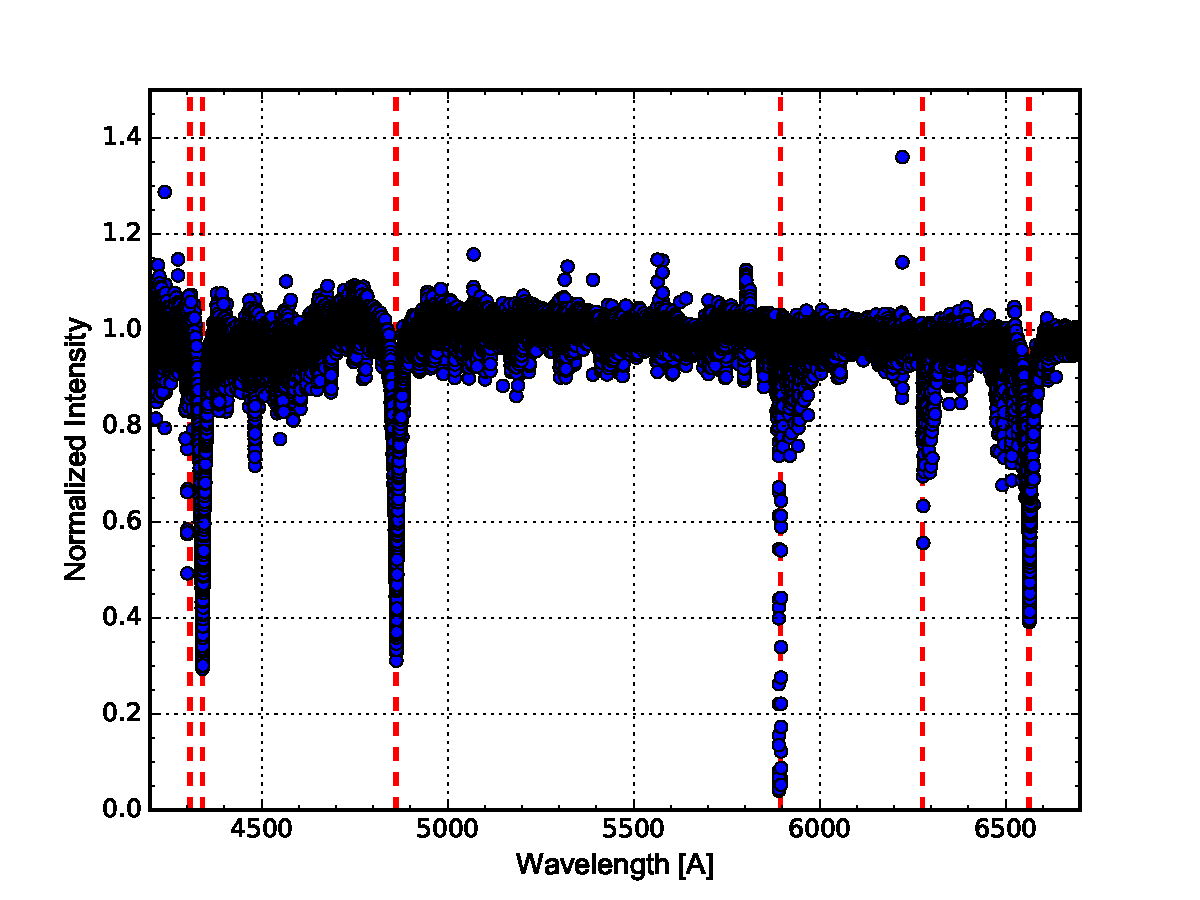
\includegraphics[scale=0.6]{absorption.pdf}%\quad
  \caption{A full stellar spectrum from 4200\,\AA\,to 6200\,\AA. The largest absorption features were indicated with red dashed lines.}
  \label{absorption}
\end{figure*}

Along with the six elements included in this study, the radial velocities, provided in table\,\ref{spectable}, were also calculated. Radial velocity\,(V) calculations were conducted with the speed of light\,(c), the literature element peak wavelength\,($\lambda$), and the shifted element peak wavelength\,($\Delta \lambda$), shown in equation\,\ref{radvel}.

\begin{equation}
V = \frac{c\Delta\lambda}{\lambda}
\label{radvel}
\end{equation}


\begin{deluxetable}{cccccccccc}
\tablecaption{Elemental Absorptions in Spectrum \label{tab:mathmode}}
\tablecolumns{3}
\tablenum{3}
\tablewidth{0pt}
\tablehead{
\colhead{Element}  & \colhead{Wavelength} & \colhead{Gaussian Peak} & \colhead{Radial Velocity}\\
& \colhead{[\AA]} & \colhead{[\AA]}  & \colhead{[km/s]} }
\centering
\startdata
Mg II & 4481.228 & 4481.9 & 	44.95654579	\\
Fe II & 4508.27  & 4508.97 &	46.54883594	\\
N V & 4603.73    & 4604.64 &	59.25871777	\\
O V & 5114.07    & 5115.09 &	59.7935318 	\\
C IV & 5801.33   & 5802.42 &	56.32739031	\\
C IV & 5811.98   & 5813.1 & 	57.77162911
\enddata
%\tablenotetext{a}{At exposure start.}
\tablecomments{Elements with the literature wavelengths. The literature values were subtracted with the modulus of the measured intensity peaks for radial velocity measurements.}
\label{spectable}
\end{deluxetable}


\begin{figure*}[ht]
  \centering
  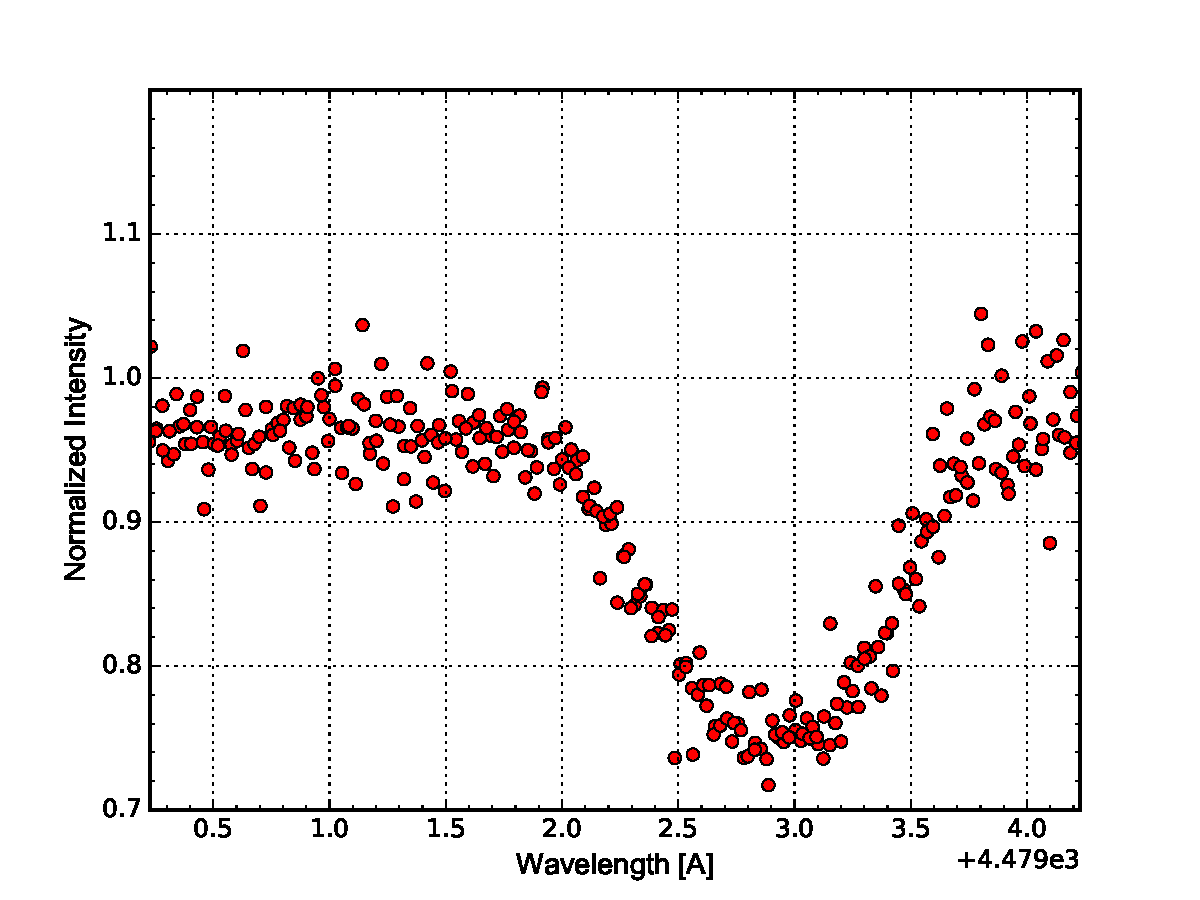
\includegraphics[scale=0.3]{mgII.pdf}%\quad
  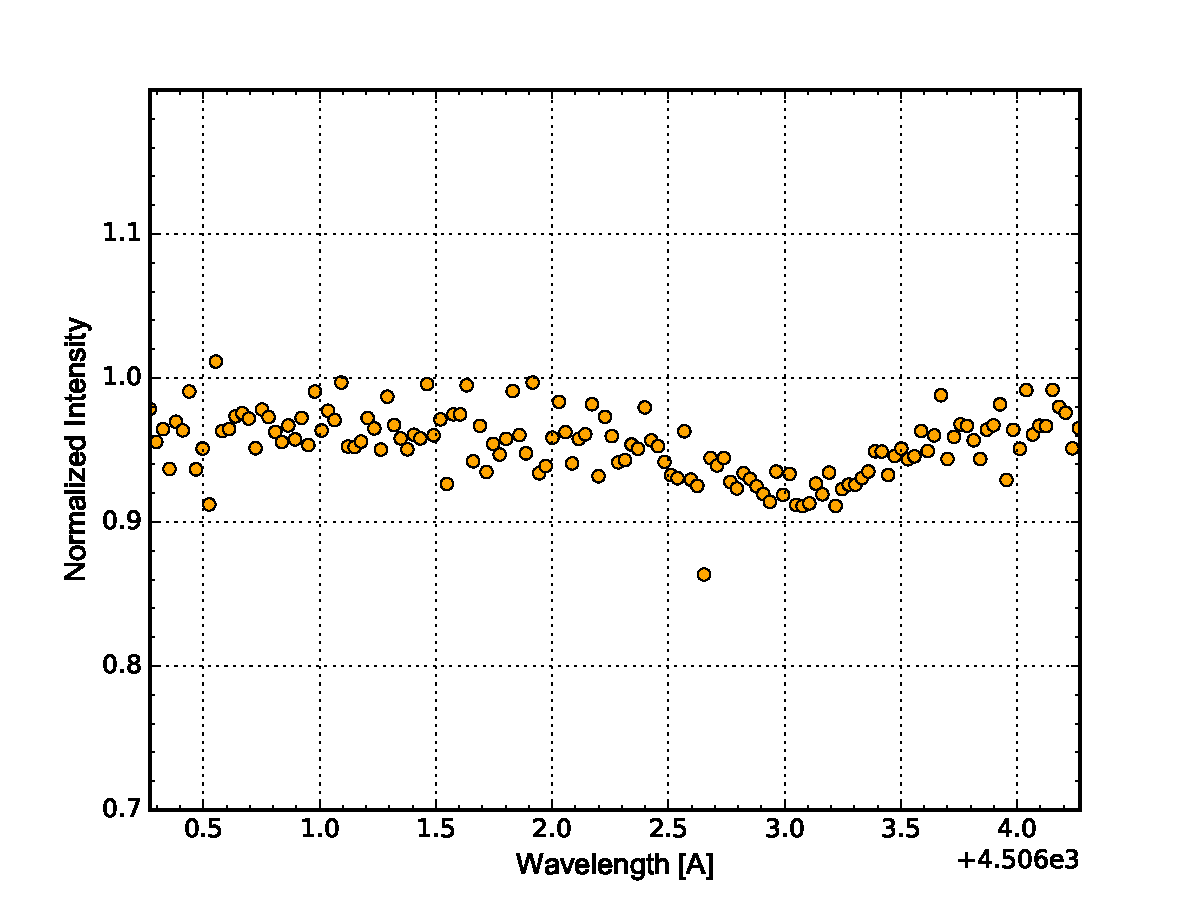
\includegraphics[scale=0.3]{feII.pdf}%\quad
  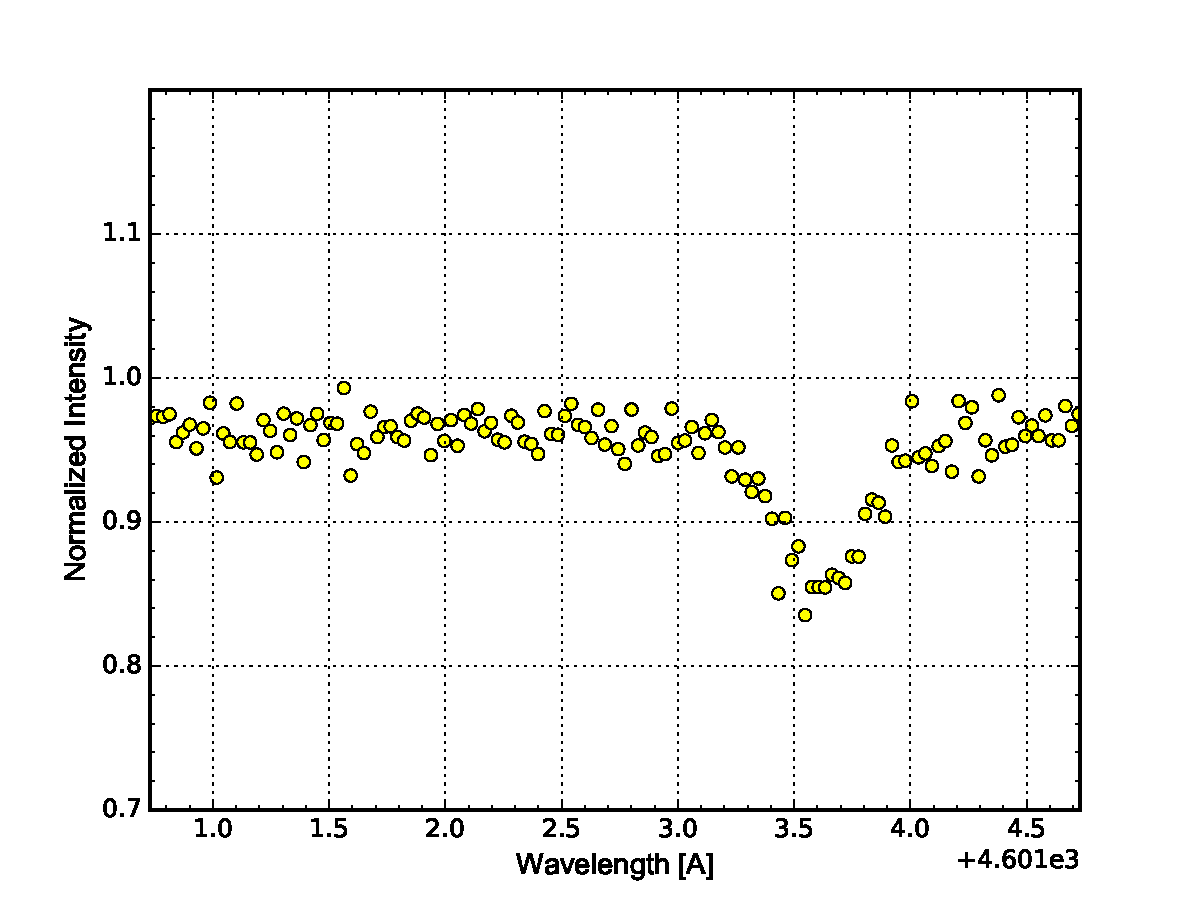
\includegraphics[scale=0.3]{nV.pdf} \\%\quad
  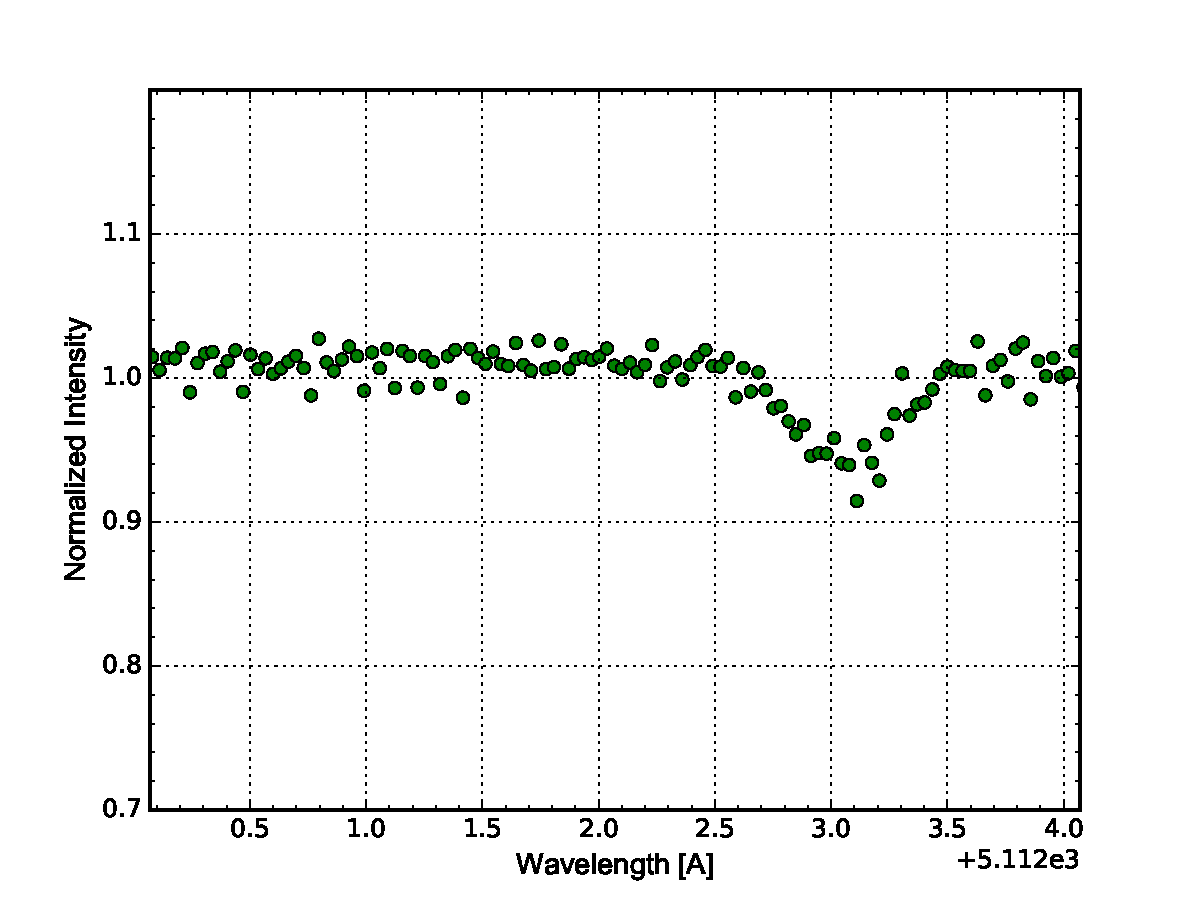
\includegraphics[scale=0.3]{oV.pdf}%\quad
  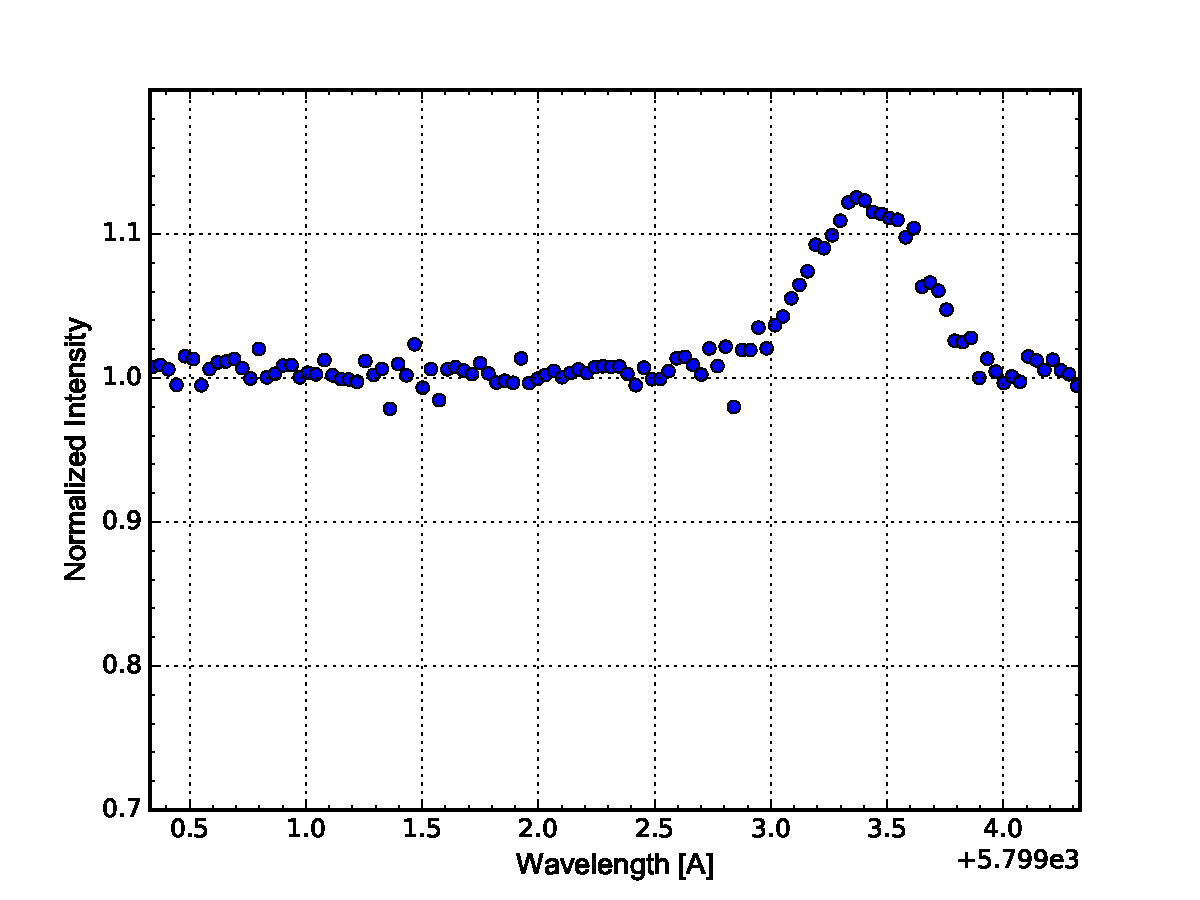
\includegraphics[scale=0.3]{cIV.pdf}%\quad
  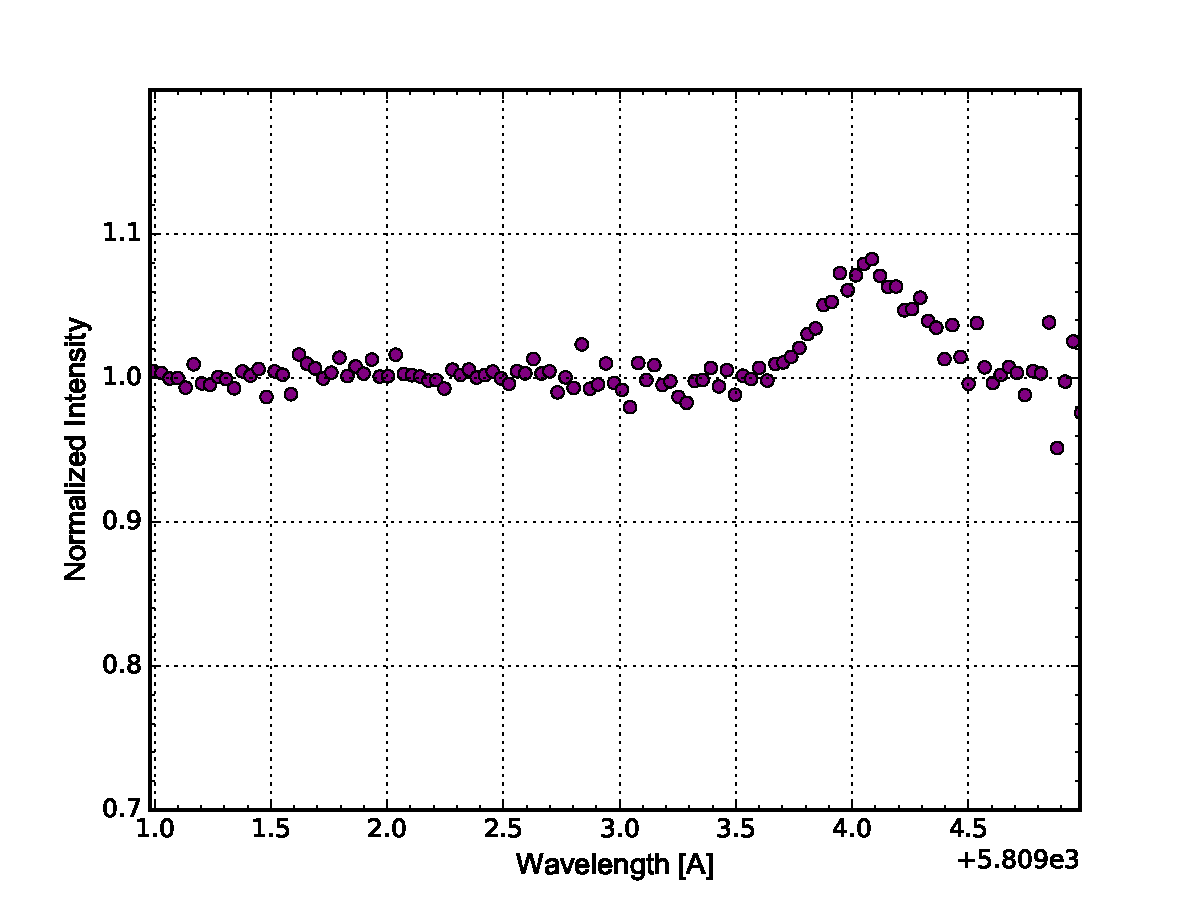
\includegraphics[scale=0.3]{cIV_2.pdf}%\quad


  \caption{Spectral features for Mg II\,(red), Fe II\,(orange), N V\,(yellow), O V\,(green), C IV\,(blue), C IV\,(purple). As the intensities are normalized, positive or negative peak, relative to the background, shows absorption or emission traits.}
  \label{distancevel}
\end{figure*}

\clearpage
Figure\,\ref{mggaus}\,(left) shows a Gaussian fit of the Mg II absorption feature. To compare to the instrumental profile, the Gaussian will be compared to the instrumental fit in equation\,\ref{inst}. The full width at half-maximum in this case will be equal to $\lambda / R$. The variable $\lambda$ will be the literature value for Mg II, 4481.228\,\AA. Additionally, the spectral resolution, R, of the Canada-France-Hawaii Telescope on Mauna Kea is 68000. 

\begin{equation}
I(x) = \exp{-\frac{x^2}{2\sigma^2}}
\label{inst}
\end{equation}


\begin{figure*}[ht]
  \centering
  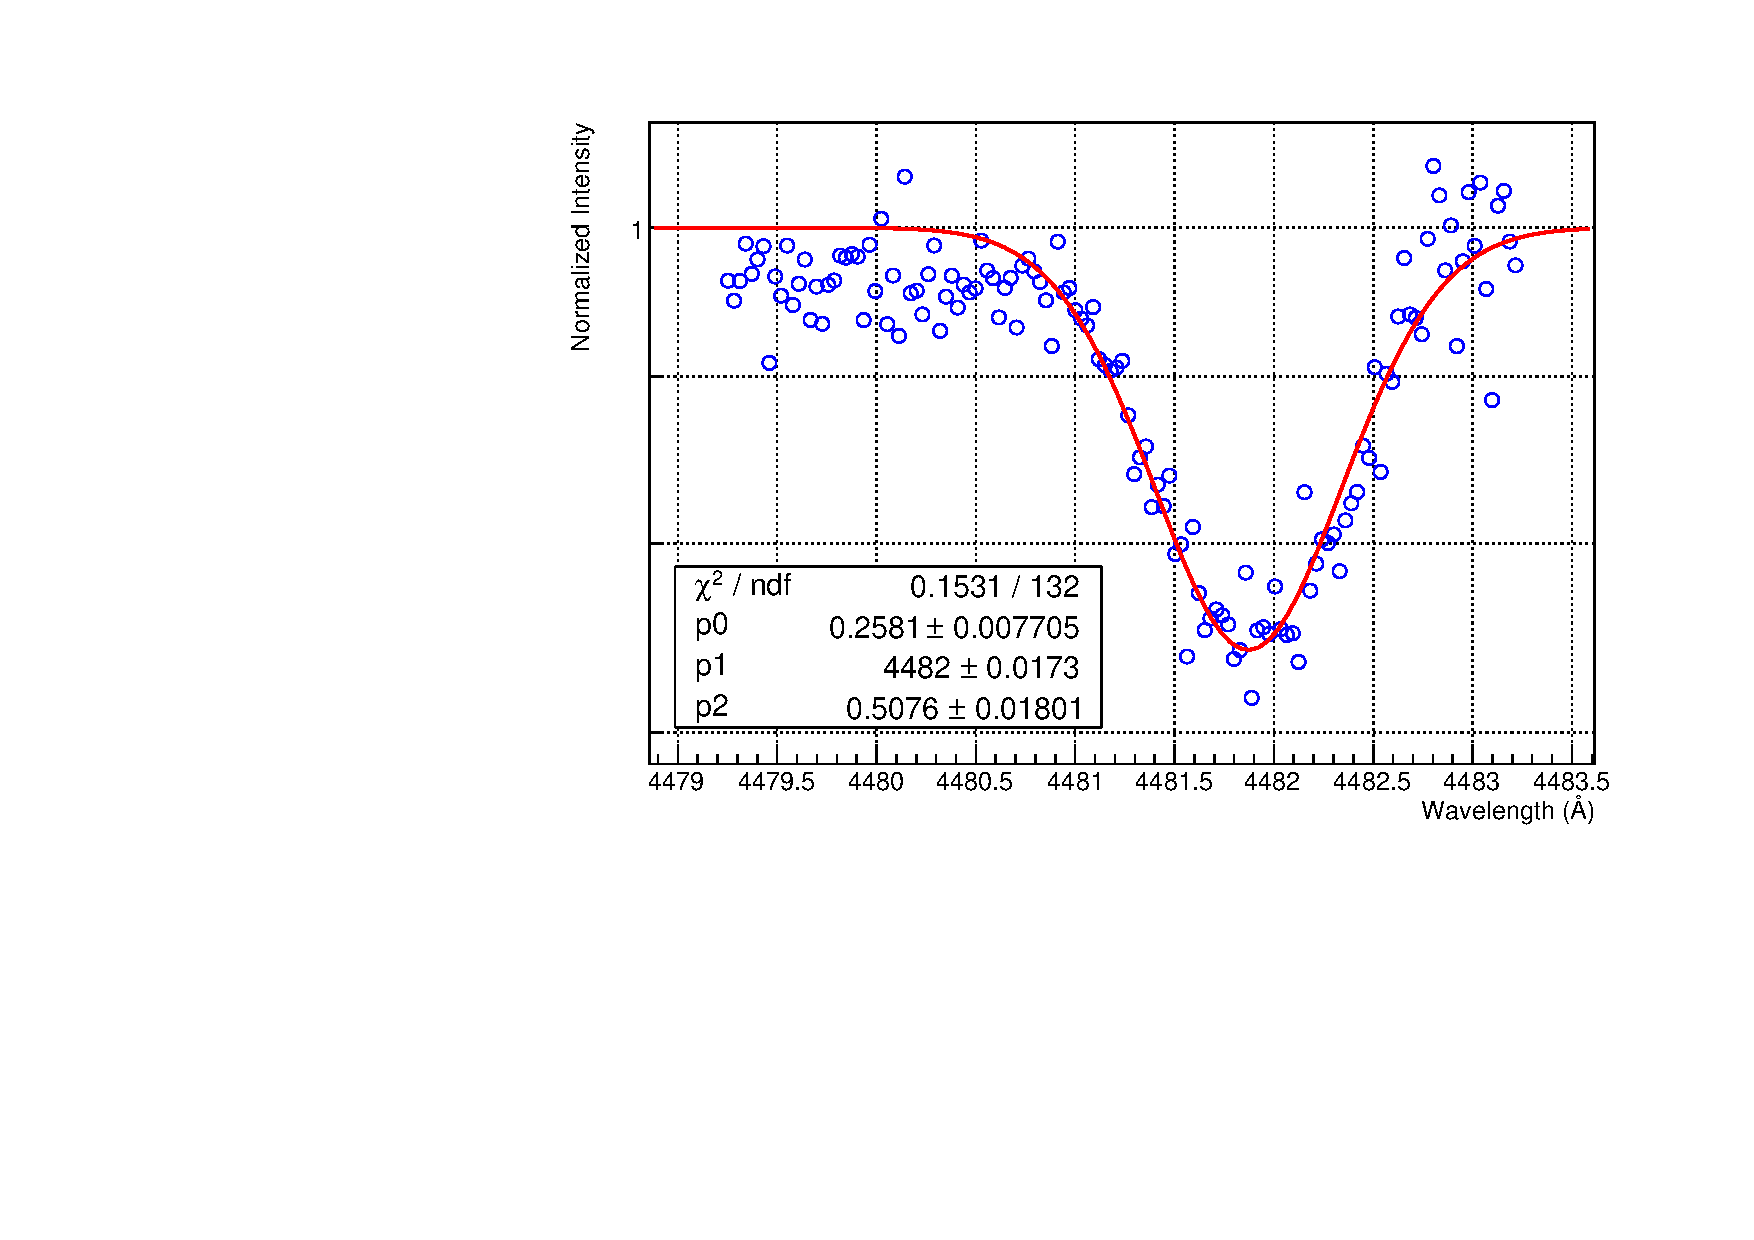
\includegraphics[scale=0.4]{mggaus.pdf}%\quad
  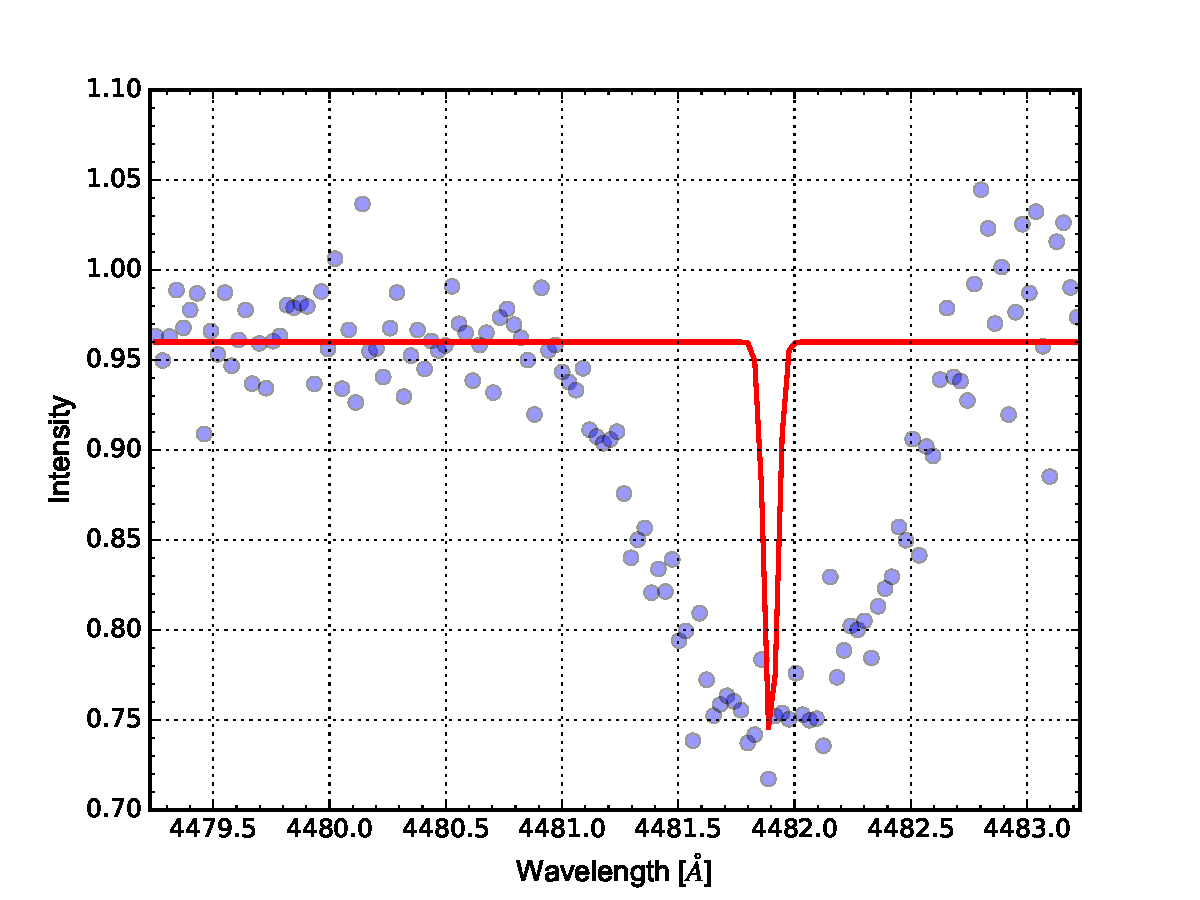
\includegraphics[scale=0.4]{Mg_absorp.pdf}%\quad
  \caption{\textbf{Left: } stellar spectrum for Mg II is shown with a Gaussian fit. \textbf{Right: } The stellar spectrum for Mg II is shown with the instrumental profile.}
  \label{mggaus}
\end{figure*}


Figure\,\ref{mggaus}\,(right) shows the less broadened spectra. It is clear that the FWHM in this scenario is far reduced compared to the fuller profile in figure\,\ref{mggaus}. The most probable extra broadening could be attributed to "Macroscopic Doppler Broadening" for this object. Radial velocities included a discrepancy of more than 10\,\AA\, between the six elements, therefore there may exist a variable line-of-sight velocity of the object.

\section{Conclusion}
The Boltzmann and Saha equations showed that the population of the first exited state hydrogen atoms does increase with increasing temperatures. The slight discrepancy for the Saha equations when varying mass density by decreasing a magnitude, was an inverse relation of population increase by a magnitude.
\\
\indent The strongest absorptions of the provided stellar spectrum included hydrogen, oxygen, sodium, and iron. The most intense absorption was the sodium line followed closely by the hydrogen lines. Probing the six elements with the respective wavelengths yielded shifted intensity peak and correlating radial velocities.
\\
\indent Finally, the instrumental broadening is far less prominent than the actual Gaussian fit. This effect was concluded to be less broad due to Macroscopic Doppler Broadening due to the varying radial velocities shown.

\section{Addendum}
Discerning between the two objects were quite trivial as hints to two different species first arose from the radial velocities. In table\,\ref{spectable}, Two of the spectral lines exhibit radial velocities near 45\,km/s and the remainder exhibit velocities at approximately 57\,km/s. Since the resolution of the telescope is very fine at 68000, the velocities would not be close within the margin of error. Secondly, another hint arises out of the difference in evolution. The Mg and Fe are both early types are type II's, whereas the N, O, and C are type IV's and V's. Due to the spectral line elemental features, these objects are most likely stars, as C-N-O is present in many late type stars, and Fe-Mg can also be produced in early types.
\\
\indent The two possibilities for the setup of these stars are possibly 1) a binary system or 2) an optical anomaly, being one star is much further away from the other.. The supporting claim is that the discrepancy in radial velocities means that they are of two differing objects. The second possibility is currently more probable due to the short time interval. To distinguish between the two possibilities, the radial velocities must be probed for the two objects for a longer period of time.





%\acknowledgments



\vspace{5mm}

\begin{thebibliography}{}


\bibitem[Hearnshaw (1986)]{1}
Hearnshaw, J.B. (1986). The analysis of starlight. Cambridge: Cambridge University Press. ISBN 0-521-39916-5.


\end{thebibliography}


\section{Appendix}

Source code for generating all data and plots will be provided in external files\,(hw2.py, flux.cpp).






%% Appendix material should be preceded with a single \appendix command.
%% There should be a \section command for each appendix. Mark appendix
%% subsections with the same markup you use in the main body of the paper.

%% Each Appendix (indicated with \section) will be lettered A, B, C, etc.
%% The equation counter will reset when it encounters the \appendix
%% command and will number appendix equations (A1), (A2), etc.


%% The reference list follows the main body and any appendices.
%% Use LaTeX's thebibliography environment to mark up your reference list.
%% Note \begin{thebibliography} is followed by an empty set of
%% curly braces.  If you forget this, LaTeX will generate the error
%% "Perhaps a missing \item?".
%%
%% thebibliography produces citations in the text using \bibitem-\cite
%% cross-referencing. Each reference is preceded by a
%% \bibitem command that defines in curly braces the KEY that corresponds
%% to the KEY in the \cite commands (see the first section above).
%% Make sure that you provide a unique KEY for every \bibitem or else the
%% paper will not LaTeX. The square brackets should contain
%% the citation text that LaTeX will insert in
%% place of the \cite commands.

%% We have used macros to produce journal name abbreviations.
%% \aastex provides a number of these for the more frequently-cited journals.
%% See the Author Guide for a list of them.

%% Note that the style of the \bibitem labels (in []) is slightly
%% different from previous examples.  The natbib system solves a host
%% of citation expression problems, but it is necessary to clearly
%% delimit the year from the author name used in the citation.
%% See the natbib documentation for more details and options.


\end{document}

%% End of file `sample.tex'.
